\newpage
\section{\ruby{付録}{ふ|ろく}:センサー\ruby{紹介}{しょう|かい}}\label{sensor_intr}
\subsection{デジタル出力\ruby{装置}{そう|ち}}

\newlength{\colF}
\setlength{\colF}{0.25\columnwidth}
\newlength{\colG}
\setlength{\colG}{0.65\columnwidth}
\newlength{\colH}
\setlength{\colH}{0.1\columnwidth}
\newlength{\colI}
\setlength{\colI}{0.35\columnwidth}

\subsubsection{LED}\label{LED}
\begin{table}[H]
	\begin{tabular}{|p{\colF}|p{\colG}|}	\hline
	\ruby{名称}{めい|しょう} & LED(えるいーでぃー)\\ \hline
	\ruby{接続箇所}{せつ|ぞく|か|しょ} & デジタルコネクタ (3pin)\\ \hline
	\ruby{機能概要}{き|のう|がい|よう} & LEDを点灯させる\\ \hline
  \end{tabular}
\end{table}

\begin{table}[H]
	\begin{tabular}{|p{\colF}|p{\colG}|}	\hline
	サンプルコードの場所 & 05/digout.hsp\\ \hline
	raspiへの入力 & なし\\ \hline
	raspiへの入力方法 & なし\\ \hline
	raspiからの出力 & \ruby{値}{あたい}が1の時点灯、値が0の時消灯\\ \hline
	raspiからの出力方法 & gpio GPIO番号, パラメータ\\ \hline
  \end{tabular}
\end{table}

\begin{table}[H]
	\begin{tabular}{|p{\colF}|p{\colG}|} \hline
	使い道 & 照明、信号機、車のライト\\ \hline
	\ruby{注意事項}{ちゅう|い|じ|こう} & なし\\ \hline
	\ruby{補足}{ほ|そく} & プラスとマイナスの電荷がLEDチップ内で\ruby{衝突}{しょう|とつ}するエネルギーを利用して発光します。LEDの光の色はLEDチップに\ruby{含}{ふく}まれている\ruby{半導体}{はん|どう|たい}の種類で決まっています\\ \hline
  \end{tabular}
\end{table}

\begin{figure}[H]
	\begin{tabular}{|p{\colH}|p{\colI}|p{\colH}|p{\colI}|} \hline
	外観 & 
	\begin{minipage}[t]{\linewidth}
    \smallskip
      \centering
      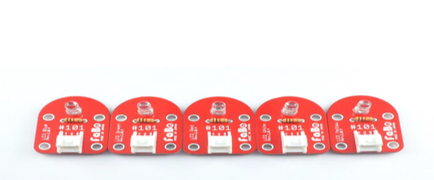
\includegraphics[width=0.8\linewidth]{images/chap05/text05-img016.png}
      \caption{LED}
      \smallskip
    \end{minipage} &
    回路記号 & 
    \begin{minipage}[t]{\linewidth}
    \smallskip
      \centering
      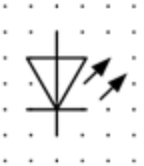
\includegraphics[width=0.3\linewidth]{images/chap05/text05-img043.png}
      \caption{LEDの回路図}
      \smallskip
    \end{minipage}\\ \hline
  \end{tabular}
\end{figure}
